\documentclass{beamer}

%Comentar a linha acima e descomentar as 3 linhas abaixo para gerar 4 slides por página do PDF.
%\documentclass[handout]{beamer}
%\usepackage{pgfpages}
%\pgfpagesuselayout{4 on 1}[a4paper, border shrink=5mm]

\usepackage[utf8]{inputenc}
\usepackage[portuguese,brazil]{babel}
\usepackage[T1]{fontenc}
\usepackage{verbatim}
\usepackage{amsmath}
\usepackage{amsfonts}
\usepackage{amssymb}
\usepackage{algorithm2e}

\usepackage{color}
\definecolor{Red}{rgb}{1.0, 0.0, 0.0}

\usepackage{url}

\usetheme[secheader]{Madrid}

\author[]{Bruno Caricchio Buss\\Lucas Pierezan Magalhães}
\institute[COS756 - UFRJ]{Universidade Federal do Rio de Janeiro}
\title[Tracking De Uma Bola]{Tracking De Uma Bola Em Um Jogo De Futebol}

\begin{document}

\begin{frame}
\titlepage
\end{frame}

\begin{frame}
\frametitle{Como achar um padrão circular?}

\vfill
Ideia: Transformada Circular de Hughes

\begin{itemize}
\item Esquema de votação do espaço das arestas.
\end{itemize}

\vfill

\begin{center}
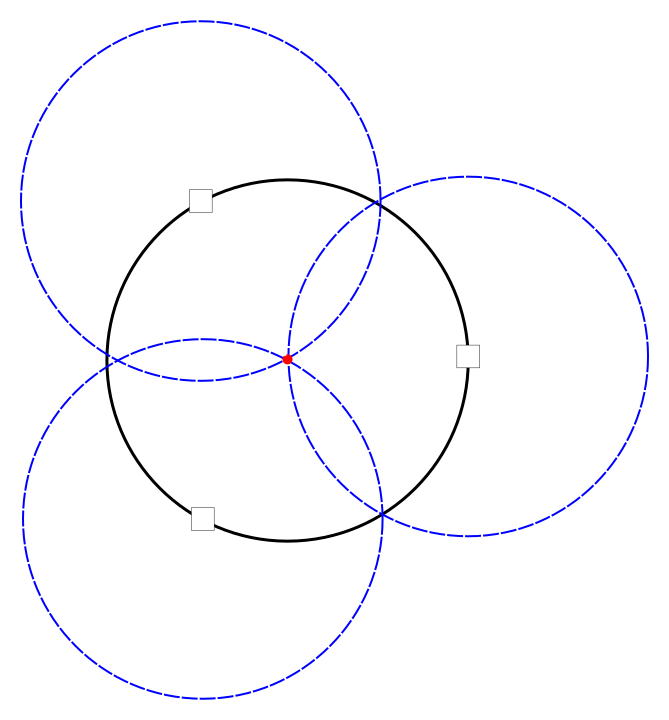
\includegraphics[scale=0.2,keepaspectratio=true]{circulos_Hughes.pdf}
\end{center}

\vfill

\end{frame}


\begin{frame}
\frametitle{Como achar um padrão circular?}

\vfill

Procedimentos:
\begin{itemize}
\item Filtro gaussiano para redução de ruído.
\item Discretização do círculo.
\item Utilizar informação do gradiente.
\item Obter valor de votação.
\end{itemize}

\vfill

Gerar um score para a circularidade da região.

\vfill

\end{frame}

\begin{frame}
\frametitle{Tracking da bola}

\vfill

Region Of Interest:

\begin{itemize}
 \item Hipótese: Movimento contínuo.
 \item Utilizar informação do frame anterior.
\end{itemize}

\vfill

Histograma:

\begin{itemize}
 \item Hipótese: Bola homogênea, com uma cor predominante.
 \item Análise dos histogramas dos pontos mais votados.
 \item Gerar score de histograma.
\end{itemize}

\vfill

Gerar score final: circularidade + histograma.

\vfill

\end{frame}

\begin{frame}
\frametitle{Outras questões}

\vfill

Ajuste de diversos parâmetros:

\begin{itemize}
 \item Canny.
 \item Sobel.
 \item Ângulo de votação.
 \item Máscara de votação.
\end{itemize}

\vfill

Além de:

\begin{itemize}
 \item Como comparar histogramas?
 \item Como calcular o score final? Qual o treshold para o tracking?
 \item Quando desistir da ROI atual?
 \item Testar template matching.
\end{itemize}

\vfill

\end{frame}

\begin{frame}

\vfill

\begin{center} {\Huge Obrigado}
\end{center}

\vfill

\end{frame}

\end{document}
​
